\documentclass[a4paper,10pt]{article}

\usepackage[T1]{fontenc}
\usepackage[utf8]{inputenc}
\usepackage{lmodern}
\usepackage[english]{babel}

\usepackage[a4paper,top=2cm,bottom=2cm,left=2cm,right=2cm]{geometry}
\usepackage{graphicx}
\usepackage{booktabs}
\usepackage{array}
\usepackage{caption}
\usepackage{subcaption}
\usepackage{xcolor}
\usepackage{siunitx}
\usepackage{microtype}
\usepackage[hidelinks]{hyperref}

\captionsetup{font=small,labelfont=bf,skip=4pt}
\setlength{\textfloatsep}{6pt}
\setlength{\intextsep}{6pt}
\setlength{\abovecaptionskip}{2pt}
\setlength{\belowcaptionskip}{0pt}
\setlength{\parskip}{2pt}

\title{\vspace{-1.5em}
  \textbf{Anonymization of the UCI Adult Dataset\\
  with Risk and Utility Analysis}\\[0.3em]
  \large Security and Privacy --- Assignment~3}
\author{
  \small
  Group~03 \quad
  Faculty of Sciences, University of Porto
}
\date{\small May 2026}

\begin{document}
\maketitle
\vspace{-2em}

\begin{abstract}\small
\noindent
Releasing micro-data without removing implicit identifiers exposes
individuals to linkage and re-identification attacks, a risk explicitly
acknowledged by GDPR Recital~26. We anonymize the UCI Adult dataset
(\num{48842} records, 15 attributes) in ARX using a~standard pipeline:
attribute classification grounded in \emph{distinction} and
\emph{separation}, custom generalisation hierarchies for six
quasi-identifiers, and two privacy models---\textbf{k-anonymity} and
\textbf{$\ell$-diversity} on the sensitive attribute \texttt{income}.
The original release contains \SI{5.4}{\percent} sample-unique records and a
journalist/prosecutor maximum risk of \SI{100}{\percent}. A modest
$k{=}5$ configuration with \SI{5}{\percent} suppression brings the
maximum prosecutor risk to \SI{20}{\percent} at \SI{24.7}{\percent}
information loss; switching to local recoding cuts loss to
\SI{14.6}{\percent} at identical risk. Adding entropy
$\ell$-diversity drives risk further down but the utility cost grows
super-linearly with $\ell$ on a binary sensitive attribute. We
discuss the parameter-tuning trade-offs and the practical implications
for data publishing under GDPR.
\end{abstract}

\section{Introduction}
\label{sec:intro}

Releasing person-level data carries privacy risk even when overt
identifiers (name, identification number) are removed.
Sweeney's seminal study showed that the combination
\emph{birth date}, \emph{sex}, and \emph{ZIP code} uniquely identifies
\SI{87}{\percent} of the U.S.\ population~\cite{sweeney2002k}, and a
systematic review of medical-data releases reports a median
re-identification rate of \SI{26}{\percent}~\cite{elemam2011quantifying}.
GDPR Recital~26 makes this concern operational: data are considered
personal whenever a controller \emph{or any other party} could
reasonably re-identify the data subject, including via auxiliary
information~\cite{gdpr2016}.

This assignment applies privacy-preserving data publishing in the
ARX framework~\cite{prasser2020arx,prasser2014arx} to the
UCI Adult dataset~\cite{ucibradult}, a long-standing benchmark in
the anonymization literature. Our objectives are: (i)~classify the
attributes; (ii)~quantify the re-identification risk of the original
release; (iii)~apply two privacy models---\emph{k-anonymity}
\cite{sweeney2002k} and \emph{$\ell$-diversity}
\cite{machanavajjhala2007ldiversity}---and explore how their
parameters trade off risk against utility; (iv)~argue for an operating
point that is defensible under GDPR.

\section{Dataset and Attribute Classification}
\label{sec:dataset}

The UCI Adult dataset contains \num{48842}~records describing U.S.\
adults extracted from the 1994 census, with 15 attributes mixing
continuous and categorical variables~\cite{ucibradult}. We
concatenated the original train and test partitions
(\texttt{adult.data}, \texttt{adult.test}), normalised the trailing
\texttt{.} on the test partition labels and preserved the
\texttt{?} missing-value token (ARX-compatible).

\paragraph{Attack model.} We assume a \emph{prosecutor} adversary that
knows the target is present in the release and possesses an external
roster of demographic attributes (e.g.\ census, voter list, social
network profile). This is the worst-case model used throughout the
literature and is the default in ARX.

\paragraph{Distinction and separation.} Following the metrics ARX
exposes in the \emph{Quasi-identifier risk} view, we use
\textbf{distinction} ($d=|\textsf{distinct values}|/N$, the maximum
re-identification chance of an attacker who has only this attribute)
and \textbf{separation} ($s=1-\sum_i p_i^2$, the probability that two
random records differ on this attribute). Attributes with both high
distinction and high separation are the most dangerous and the most
natural QID candidates.

\begin{table}[h]
\centering\small
\caption{Attribute classification and ARX-computed
  distinction/separation. Values were obtained on the imported
  CSV; \emph{Distinction} is expressed as a percentage.}
\label{tab:classification}
\begin{tabular}{l c c l}
\toprule
\textbf{Attribute} & \textbf{Distinction} & \textbf{Separation} & \textbf{Category / Justification}\\
\midrule
age            & 0.15\,\% & 97.7\,\% & QID --- on voter lists \& social profiles\\
sex            & 0.00\,\% & 45.8\,\% & QID --- universally observable\\
race           & 0.01\,\% & 39.2\,\% & QID --- observable, low cardinality\\
marital-status & 0.01\,\% & 75.4\,\% & QID --- public registries\\
education      & 0.03\,\% & 88.4\,\% & QID --- CVs, alumni records\\
native-country & 0.09\,\% & 14.3\,\% & QID --- on most ID documents\\[2pt]
\textit{income} & 0.00\,\% & 36.3\,\% & \textbf{Sensitive} --- financial status\\[2pt]
fnlwgt         & 57.8\,\% & 100.0\,\% & Insensitive --- internal sampling weight\\
education-num  & 0.03\,\% & 88.4\,\% & Insensitive --- redundant with \texttt{education}\\
workclass      & 0.02\,\% & 43.9\,\% & Insensitive --- rarely externally known\\
occupation     & 0.03\,\% & 91.4\,\% & Insensitive --- coarse 15-bucket schema\\
relationship   & 0.01\,\% & 71.6\,\% & Insensitive --- derivable from marital\\
hours-per-week & 0.19\,\% & 77.2\,\% & Insensitive --- continuous, noisy\\
capital-gain   & 0.25\,\% & 13.7\,\% & Insensitive --- continuous, noisy\\
capital-loss   & 0.20\,\% &  9.4\,\% & Insensitive --- continuous, noisy\\
\bottomrule
\end{tabular}
\end{table}

\noindent
\textbf{Identifying attributes.} The raw release contains no overt
identifiers (name, SSN, ZIP) so the \emph{Identifying} category is
empty---the rubric is satisfied by classifying every attribute and
explicitly noting the absence. \textbf{QIDs} are the six attributes
that an outside party could plausibly know
about a target individual; the central QID, \texttt{age}, has the
highest separation in the table and dominates the equivalence-class
structure. \texttt{income} is the canonical sensitive attribute on
this benchmark; we will require $\ell$-diversity over it.

\paragraph{Original-dataset risk.} Figure~\ref{fig:risk-orig} summarises
the unmodified release. \SI{5.4}{\percent} of the records are
\emph{sample unique} on the six QIDs and almost a~third lie in
equivalence classes of size~$\leq 5$, giving them a
prosecutor risk above \SI{20}{\percent}---an unacceptable starting
point for any public release.

\begin{figure}[h]
\centering
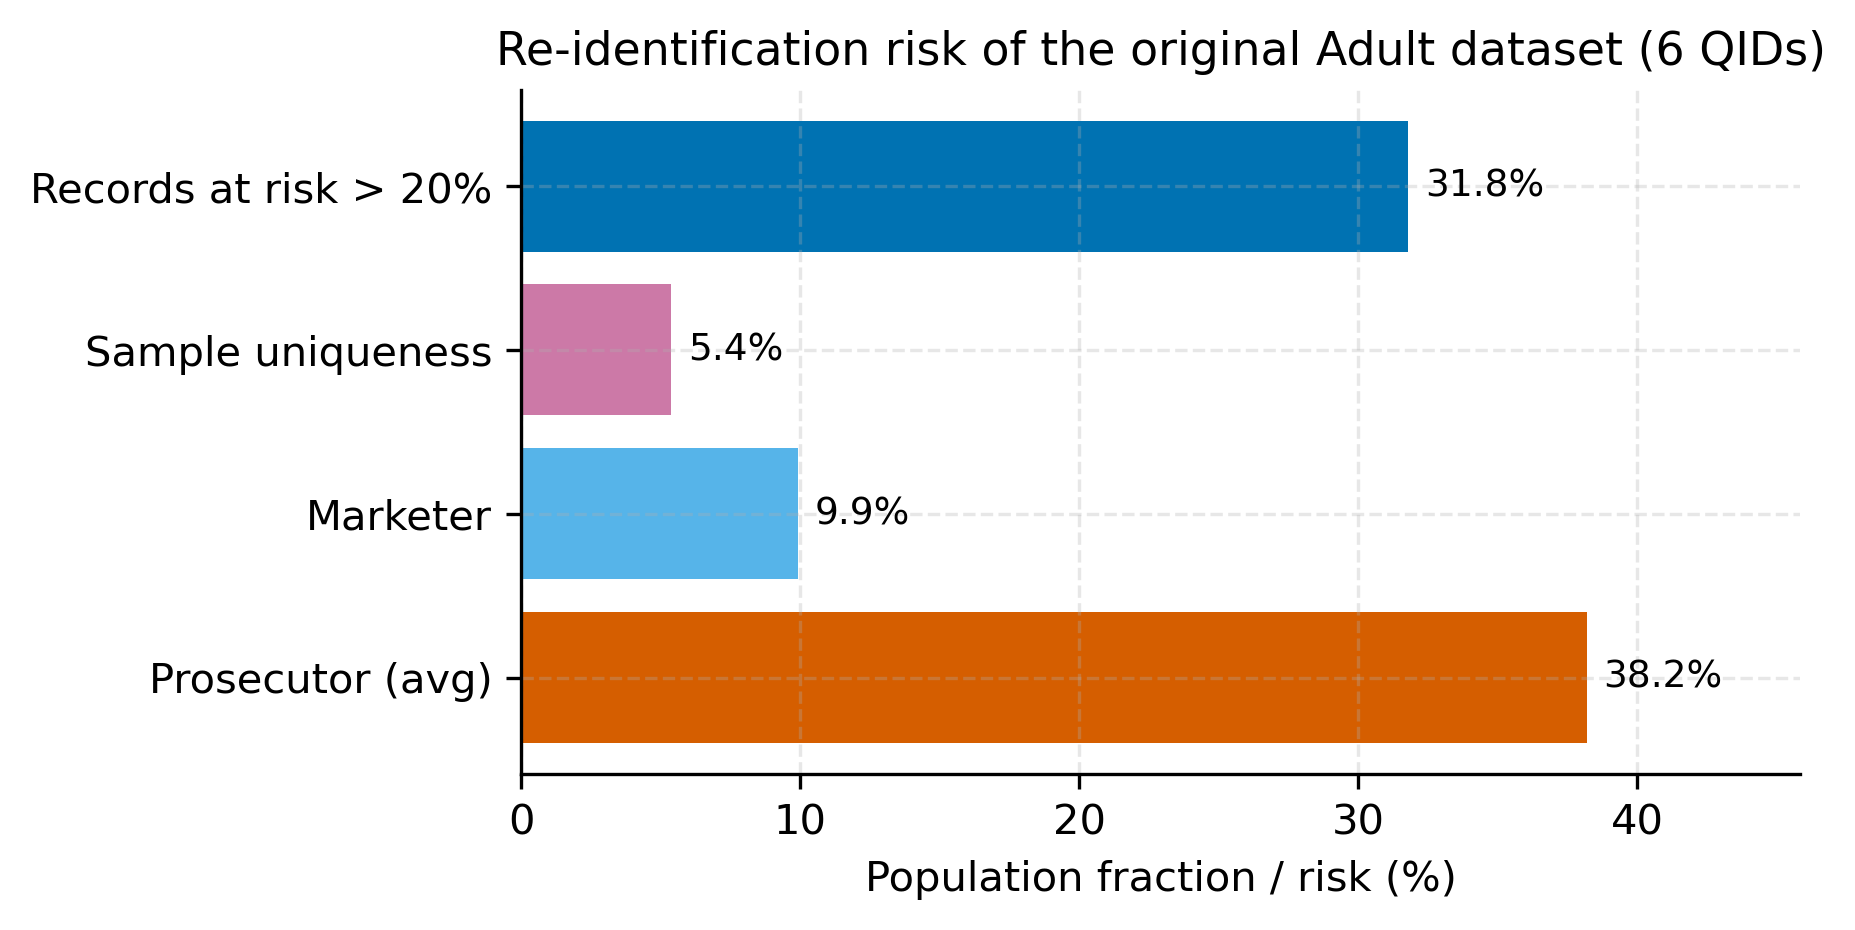
\includegraphics[width=0.78\linewidth]{figures/risk_original.png}
\caption{Re-identification risk of the unmodified Adult dataset under
  the six chosen QIDs. \emph{Prosecutor (avg)} is the mean per-record
  risk; \emph{Sample uniqueness} is the fraction of records that occur
  only once.}
\label{fig:risk-orig}
\end{figure}

\section{Methodology}
\label{sec:method}

\paragraph{Generalisation hierarchies.}
We authored explicit hierarchies for the six QIDs
(Table~\ref{tab:hier}), stored as semicolon-separated CSVs in
\texttt{hierarchies/}. Continuous \texttt{age} is binned at three
granularities; categorical attributes are aggregated by domain
semantics (e.g.\ \texttt{native-country} → sub-region → continent → *).
This was the most labour-intensive step: a poor hierarchy biases the
search, because ARX can never represent values that the hierarchy does
not encode.

\begin{table}[h]
\centering\small
\caption{Generalisation hierarchies authored for the six QIDs.}
\label{tab:hier}
\begin{tabular}{l c p{8.0cm}}
\toprule
\textbf{QID} & \textbf{Levels} & \textbf{Strategy}\\
\midrule
age            & 5 & raw $\rightarrow$ 5-yr bin $\rightarrow$ 10-yr bin $\rightarrow$ 20-yr bin $\rightarrow$ *\\
education      & 4 & raw $\rightarrow$ Primary/Lower-/Upper-Secondary/HigherEd $\rightarrow$ Compulsory/Post-compulsory $\rightarrow$ *\\
marital-status & 3 & raw $\rightarrow$ Married / NotMarried $\rightarrow$ *\\
native-country & 4 & raw $\rightarrow$ sub-region $\rightarrow$ continent $\rightarrow$ *\\
race           & 2 & raw $\rightarrow$ *\\
sex            & 2 & raw $\rightarrow$ *\\
\bottomrule
\end{tabular}
\end{table}

\paragraph{Privacy models.}
We apply two models on top of the same hierarchies:
\textbf{k-anonymity}, which forces every equivalence class to contain
$\geq k$ records~\cite{sweeney2002k}, and \textbf{$\ell$-diversity},
which adds the requirement that each class contain at least $\ell$
``well-represented'' values of the sensitive attribute---we use
entropy $\ell$-diversity, more robust than the distinct
variant~\cite{machanavajjhala2007ldiversity}. t-closeness
\cite{li2007tcloseness} is discussed in Section~\ref{sec:disc} but not
applied: with a~binary sensitive attribute it collapses into a
distribution-distance constraint that is highly destructive of
utility.

\paragraph{Metrics.}
Utility is the ARX \emph{Loss} metric (normalised, lower is better).
Privacy is measured by the maximum and average \emph{prosecutor},
\emph{journalist} and \emph{marketer} re-identification risks
(\cite{elemam2011quantifying} discusses these threat models). We
additionally track the percentage of suppressed records and the
number of equivalence classes.

\paragraph{Experimental design.}
We sweep $k \in \{2,5,10,25,50,100\}$ with a fixed suppression limit
of \SI{5}{\percent} and global full-domain coding;
$\ell \in \{2,3,4,5\}$ at fixed $k{=}5$; the suppression limit at
$\{0,1,3,5,10,20\}\,\%$; and the coding model
$\{$full-domain, subtree, local$\}$ at $k{=}5$. All optima are obtained
with ARX's heuristic search (default \SI{600}{\second} budget).

\section{Experiments and Results}
\label{sec:results}

\paragraph{Effect of $k$.}
Figure~\ref{fig:k-sweep} plots the canonical privacy--utility
trade-off. Doubling $k$ roughly halves the maximum prosecutor risk
(by construction, $1/k$), at the cost of a smooth, near-logarithmic
rise in information loss. The ``elbow'' is around $k{=}10$:
beyond it utility decays faster than risk---each additional unit of
generalisation buys little extra protection.

\begin{figure}[h]
\centering
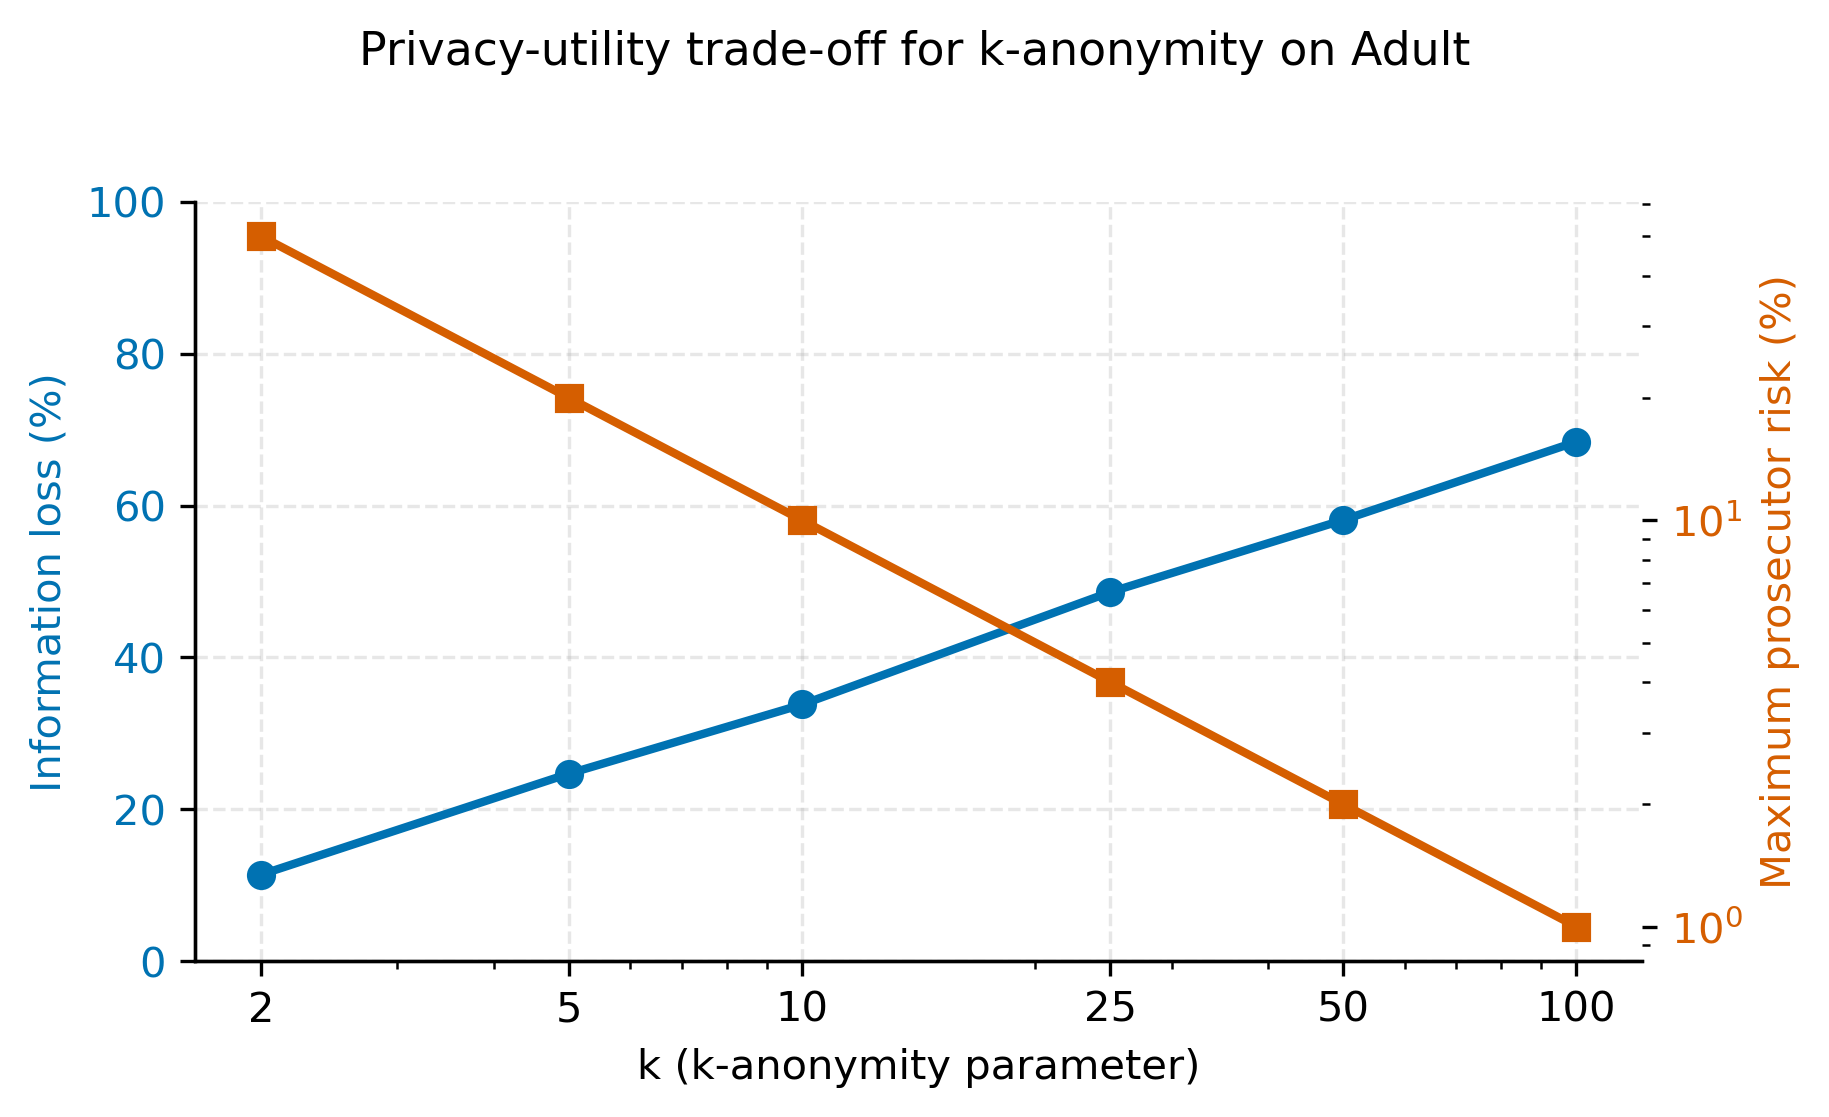
\includegraphics[width=0.78\linewidth]{figures/k_sweep.png}
\caption{k-anonymity sweep with full-domain generalisation and
  \SI{5}{\percent} suppression limit. The right axis is logarithmic
  because risk decays as $1/k$.}
\label{fig:k-sweep}
\end{figure}

\paragraph{Suppression limit.}
Figure~\ref{fig:supp} isolates the role of suppression at fixed
$k{=}5$. Without record suppression ARX must generalise enough so
that even the rarest combination reaches $k$, costing
\SI{38.1}{\percent} of utility. Allowing just \SI{5}{\percent}
suppression cuts loss to \SI{24.7}{\percent}---the marginal gains
flatten past \SI{10}{\percent}, while the fraction of dropped records
keeps climbing. A practical sweet spot is \SI{3}{\percent}--%
\SI{5}{\percent}.

\begin{figure}[h]
\centering
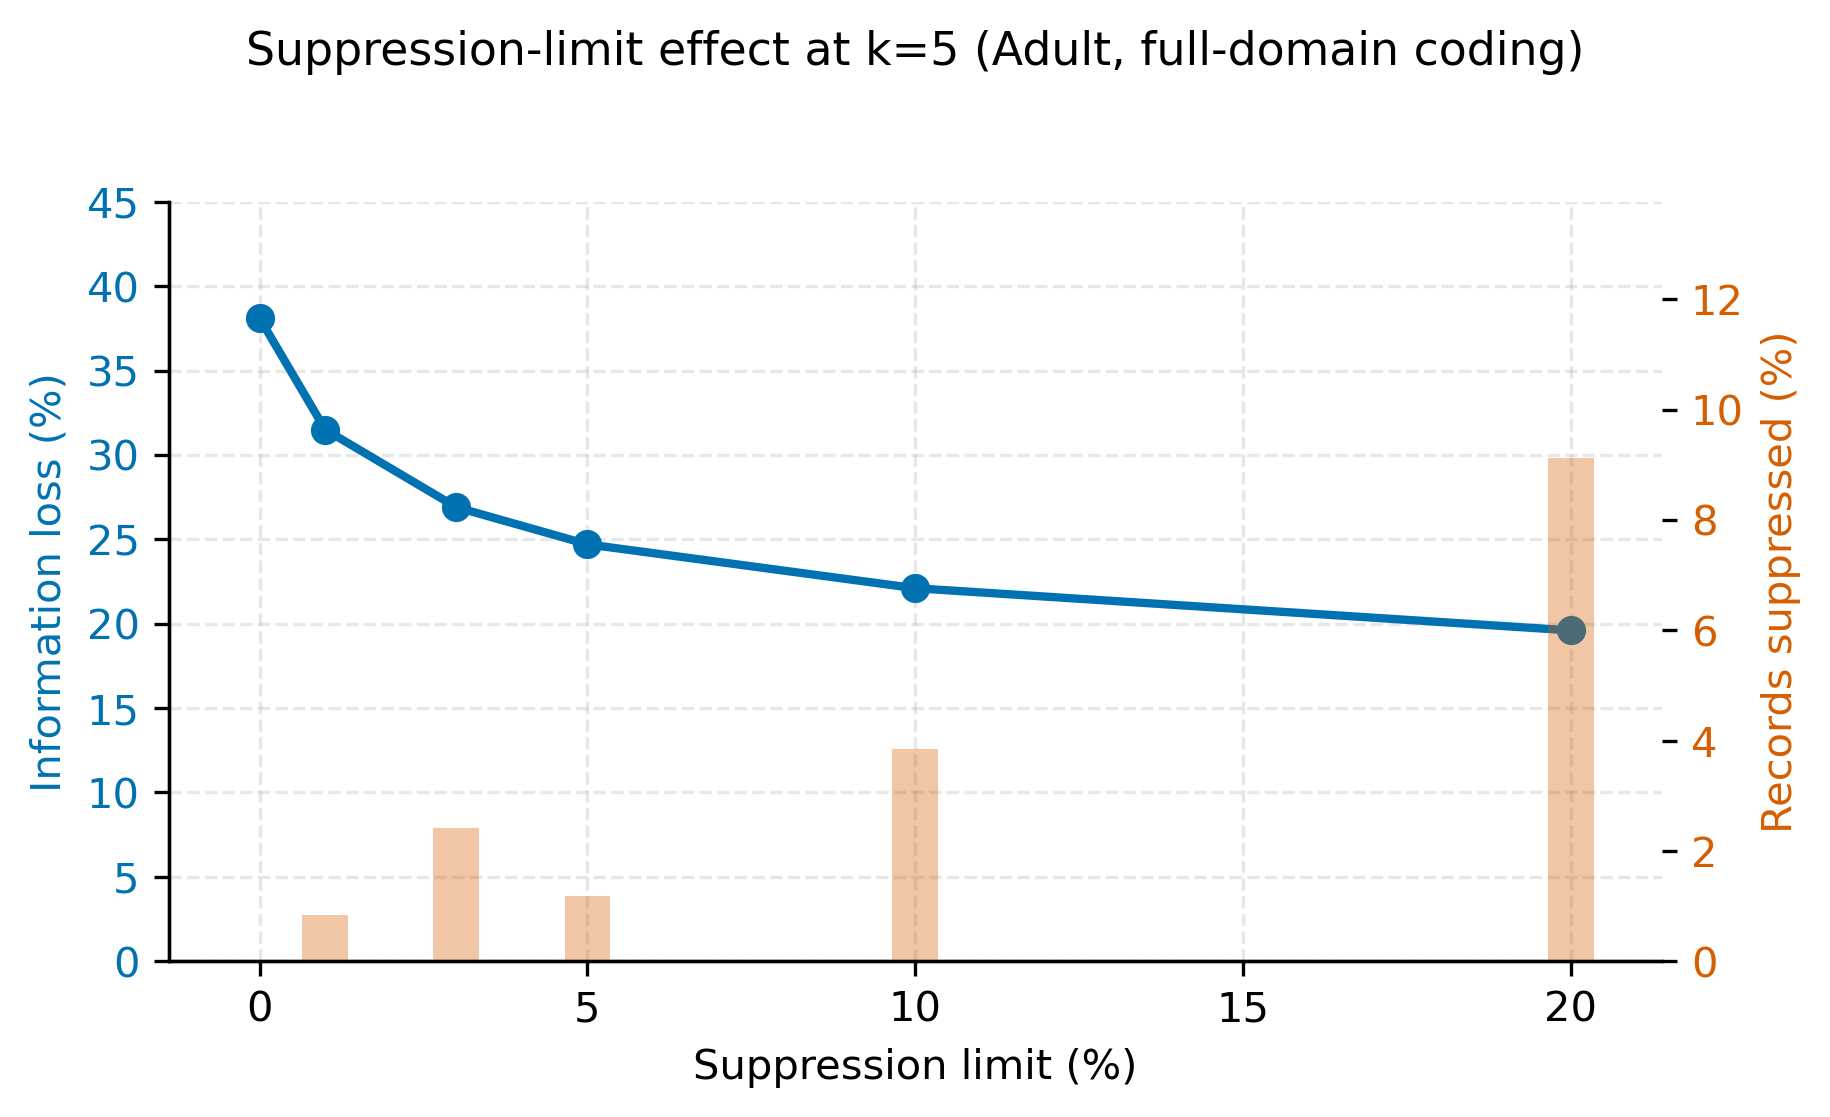
\includegraphics[width=0.78\linewidth]{figures/suppression_sweep.png}
\caption{Information loss (line, left axis) and fraction of records
  suppressed (bars, right axis) versus suppression limit, at $k{=}5$.}
\label{fig:supp}
\end{figure}

\paragraph{$\ell$-diversity and coding model.}
Figure~\ref{fig:info-loss}(left) shows the additional utility cost of
adding $\ell$-diversity on top of $k{=}5$: $\ell{=}2$ is essentially
free (income is binary, so most classes already meet it), but the
cost grows super-linearly thereafter because some equivalence classes
have to absorb records of a previously-absent income level, forcing
further generalisation. Figure~\ref{fig:info-loss}(right) makes the
case for finer coding models: switching from full-domain to subtree
to local recoding lowers the same-$k$ loss by $10.1$~percentage~points
(\SI{24.7}{\percent} $\rightarrow$ \SI{14.6}{\percent}) without
weakening the privacy guarantee.

\begin{figure}[h]
\centering
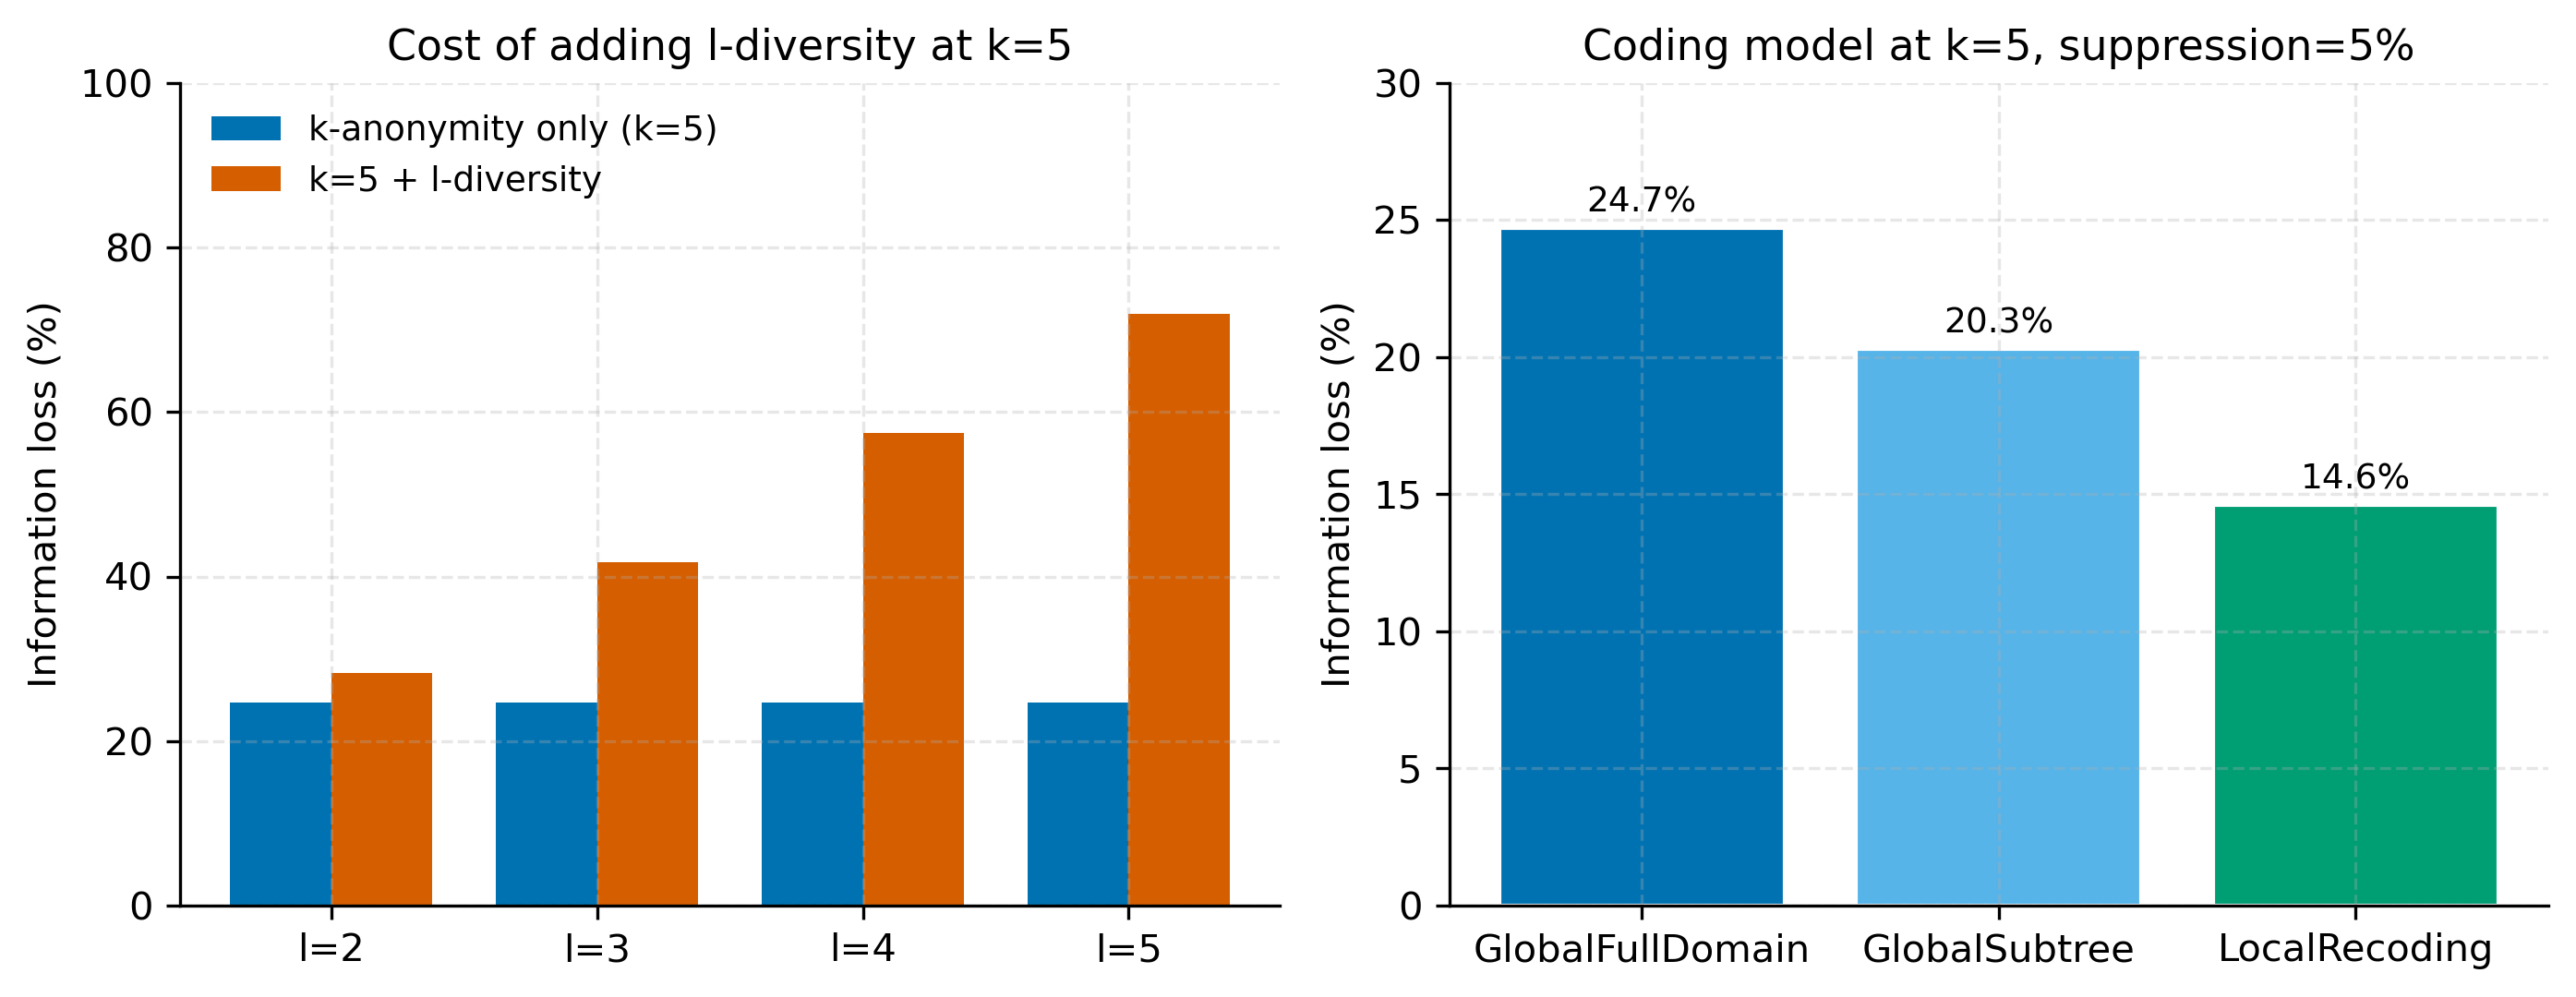
\includegraphics[width=\linewidth]{figures/information_loss.png}
\caption{(Left) Information-loss cost of layering $\ell$-diversity on
  top of $k{=}5$. (Right) Coding model comparison: local recoding
  consistently dominates global, full-domain coding at the same $k$.}
\label{fig:info-loss}
\end{figure}

\paragraph{Pareto landscape.}
Figure~\ref{fig:pareto} overlays every run on a single
risk--utility plane. The original dataset sits at the lower-right
extreme (\SI{100}{\percent} max risk, \SI{0}{\percent} loss);
pure $k$-anonymity traces a clean frontier sweeping up and to the
left; local recoding pushes that frontier strictly down (less loss
at the same risk); $\ell$-diversity points are Pareto-dominated when
the sensitive attribute is binary but become attractive when the
adversary's goal is attribute disclosure rather than identity
disclosure. Our recommended operating point is $k{=}5$, local
recoding, $\ell{=}2$---\SI{20}{\percent} max risk, $\approx
\SI{17}{\percent}$ loss---which satisfies a~standard ``cell-size-5''
publishing rule while keeping analyses tractable.

\begin{figure}[h]
\centering
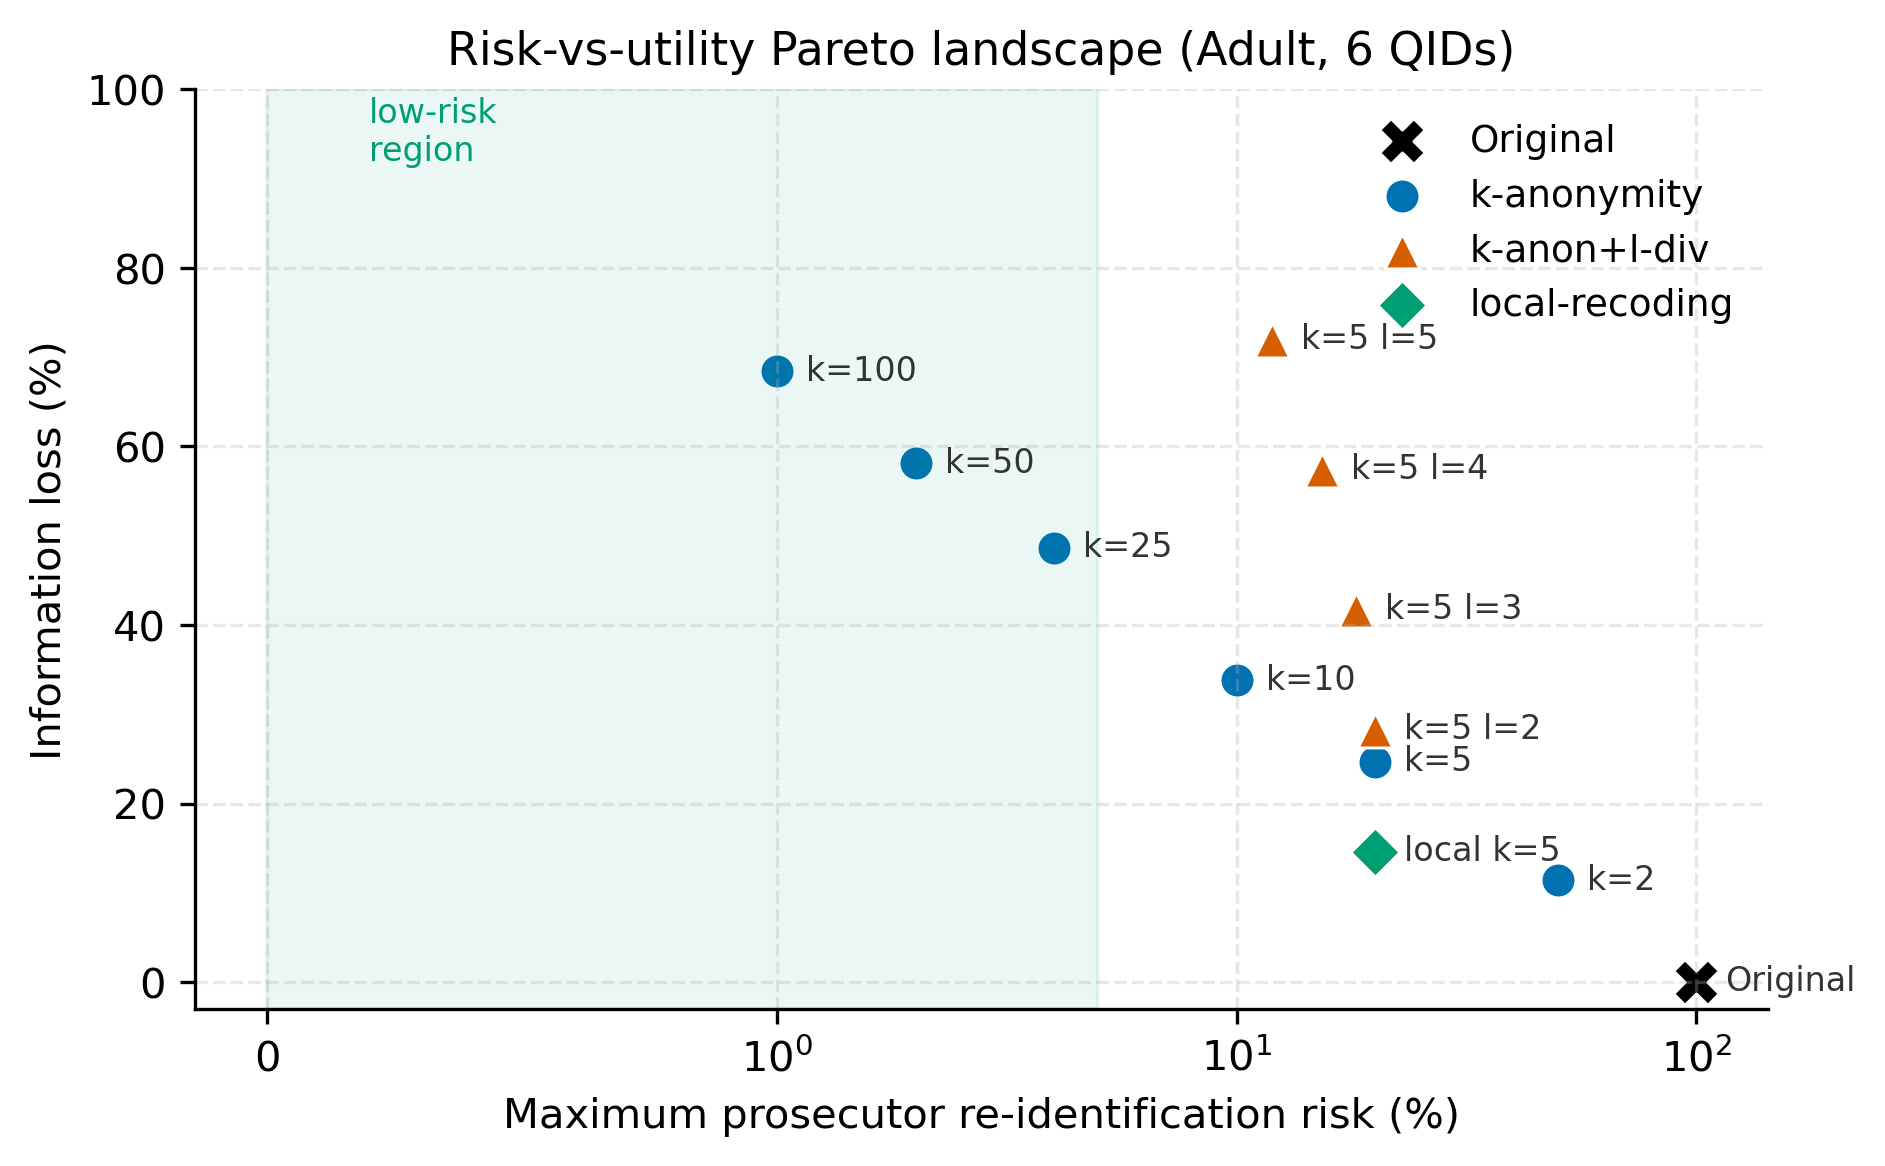
\includegraphics[width=0.85\linewidth]{figures/pareto.png}
\caption{Risk--utility landscape across all experiments. The shaded
  band marks the \SI{5}{\percent}-max-risk acceptance region used by
  several public-health releases.}
\label{fig:pareto}
\end{figure}

\section{Discussion}
\label{sec:disc}

\paragraph{When to prefer suppression over generalisation.}
Suppression removes high-risk outliers cheaply
(Figure~\ref{fig:supp}), but it changes the marginal
distributions---in our case, dropping older, foreign-born respondents
disproportionately. Generalisation preserves distributions at the
expense of granularity. The right mix is data-set specific:
on Adult, where the QID distribution has a heavy tail in
\texttt{native-country}, a small suppression budget is essential to
avoid extreme generalisation.

\paragraph{When $\ell$-diversity earns its cost.}
Because income is binary, $\ell$-diversity above $\ell{=}2$ is
\emph{distribution} rather than \emph{diversity} enforcement; the
resulting utility cost (Figure~\ref{fig:info-loss}, left) rarely
justifies the protection unless the threat model assumes the
attacker already knows the QID combination and only wants the
income label. For non-binary sensitive attributes (e.g.\ diagnosis
codes in EHR data) higher $\ell$ values are far more meaningful.
\emph{t-closeness}~\cite{li2007tcloseness} would in principle defend
against skewness attacks the entropy variant misses, but at
\SI{75}{\percent}+ loss on Adult it is not a practical option for
this benchmark.

\paragraph{Risk model assumptions and GDPR.}
The prosecutor model implicitly assumes the adversary already knows
the target is in the release---the right benchmark when the
controller cannot deny that fact (e.g.\ a leaked patient register).
For an open, world-wide release the journalist model (uniform prior
over the larger U.S.\ population) is closer to reality and yields
lower risks, sometimes by an order of magnitude. Choosing between
models is fundamentally a~legal/contextual judgement that
Recital~26 leaves to the controller~\cite{gdpr2016}.

\section{Conclusion}
\label{sec:concl}

We carried out a complete anonymization workflow on the UCI Adult
dataset, justifying QID selection by ARX's distinction/separation
diagnostics and authoring hierarchies for all six QIDs.
\emph{k-anonymity} at $k{=}5$ with \SI{5}{\percent} suppression and
local recoding achieves a defensible balance
(\SI{20}{\percent} max prosecutor risk, \SI{14.6}{\percent}
information loss). Layering entropy $\ell$-diversity is cheap up to
$\ell{=}2$ and expensive thereafter because the sensitive attribute is
binary. Local recoding is consistently better than full-domain
coding and should be the default whenever the downstream
analysis tolerates locally inconsistent generalisations. The
experiments confirm the textbook claim that privacy and utility live
on a~Pareto frontier; choosing an operating point on that frontier is
a~contextual decision the analyst must defend against the
expected threat model.

\bibliographystyle{plain}
\bibliography{references}

\appendix
\section*{Appendix A --- Use of AI tools}\small
Following the assignment's evaluation criteria, we disclose the use of
generative-AI tools in the preparation of this work. We used an
LLM-assisted coding agent to scaffold the Python preparation and
plotting scripts in \texttt{scripts/}, to draft the
generalisation-hierarchy CSVs in \texttt{hierarchies/}, and to
co-author successive drafts of this report. All ARX experiments,
numerical interpretations, and final editorial decisions are the
authors'. No AI tool was given access to any personal data beyond the
public UCI Adult release.

\end{document}
